\fancyhead[LO]{{\scriptsize {\FA \ }我们最幸福 {\FA } 结束语 等待}}%奇數頁眉的左邊
\fancyhead[RO]{{\tiny{\textcolor{Gray}{\FA \ }}}\thepage}
\fancyhead[LE]{{\tiny{\textcolor{Gray}{\FA \ }}}\thepage}
\fancyhead[RE]{{\scriptsize {\FA \ }我们最幸福 {\FA } 结束语 等待}}%偶數頁眉的右邊
\fancyfoot[LE,RO]{}
\fancyfoot[LO,CE]{}
\fancyfoot[CO,RE]{}
\chapter*{结束语 等待}
\addcontentsline{toc}{chapter}{\hspace{5mm}结束语 等待}
\vspace{15mm}
\begin{flushright}
	\textcolor{PinYinColor}{\EN \huge{Epilogue\\
	\ \\}}
\end{flushright}
\begin{figure}[!htbp]
	\centering
	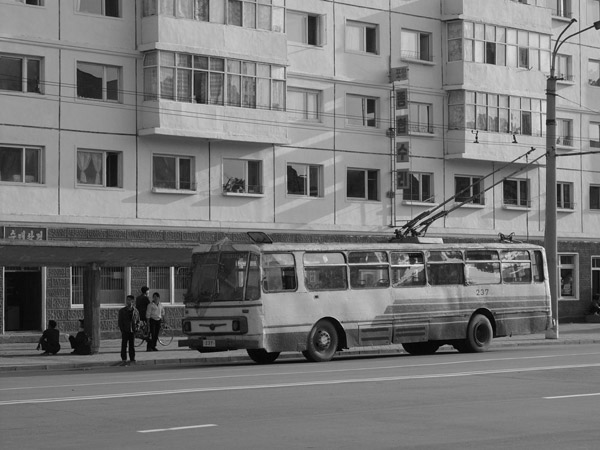
\includegraphics[width=6cm]{./Chapters/Images/21.jpg}
	\caption*{2008年清津主干道的一个公交站}
\end{figure}


在首尔为《洛杉矶时报》(Los Angeles Times)作报导的这5年期间,我参加了大量的,与一些同行、外交官和学者的宴会。无一例外,话题都会转到北朝鲜,参与者都会猜测着金正日政权什么时候会垮台。\\

北朝鲜政权残喘至今对于一些专业的北朝鲜观察家来说简直就是个神话。早至90年代,其近在眼前的覆灭被一致认为几乎是板上钉钉的事情\footnote{著名的北朝鲜学者尼古拉斯·艾伯施塔特(Nicholas Eberstadt)于1990年6月,在其专栏中发表题为《北朝鲜的崩溃即将到来》的文章。}。面对诸多质疑,北朝鲜历经柏林墙倒塌、苏联解体、中国市场化改革、金日成去世、90年代的饥荒,两届小布什(George W. Bush)总统任期后,仍然生存了下来。布什(George W. Bush)非常著名地将北朝鲜连同伊朗、伊拉克归为了“邪恶轴心”,且发誓要将金正日像他对萨达姆(Saddam Hussein)那样绳之于法。然而时至2010年,布什(George W. Bush)早已下台,而金正日虽然健康状况不佳,却仍然在位。作为20世纪最后一个独裁者,他就是一个应该被抛弃在历史尘堆里的活化石。\\

金用像在冷战高峰期一样的方式,统治着他的国家,炮制着一些夸张的宣传、禁止大部分外国人到访、用核武器和导弹威胁着或真实或臆想的敌人。北朝鲜经行过两次核试,一次在2006年、一次在2009年。美国几届政府,近20年的外交努力却未能达成协议,在该协议下北朝鲜将放弃它的核计划,而作为回报,它将获得美国外交上的承认,并签署永久的和平协议,终结朝鲜战争。\\

在本书撰写期间,南北处于90年代早期以来关系最为紧张的时期。在2010年3月26日,一声爆炸将在黄海执行任务的南韩巡逻舰天安号,炸的四分五裂。46名水兵丧生。南韩于5月20日宣布调查人员发现确凿证据证明该舰是受到北朝鲜的鱼雷攻击。威胁要以武力应对的南韩切断了对北朝鲜的所有经济援助。2007年当选的南韩保守派总统李明博终结了在金大中“阳光政策”下同北朝鲜持续了10年的经济、文化交流。一度成为北朝鲜最重要的硬通货来源的金刚山旅游项目,也于2008年北朝鲜拒绝为一次很明显的误杀南韩游客的事件中道歉后,而中止了。\\

平壤在好战的同时,经济上也强硬起来。在其它共产世界都臣服于资本主义几十年后,金正日仍然幻想着像他父亲在1950年代那样运作其经济体系。如果可以,他将把这个国家大幅度的带回过去,禁止那些让宋女士生存下来的市场化改革。\\

在过去的几年间,劳动党发布了一连串旨在收紧市场经济自然运作的愚蠢规定。除了40岁或以上的妇女,禁止其它人成为商贩;所有的男人及年轻女性都要向其工作的国有工厂报到,而不论工厂是否能发得出工资。对于什么能买、什么能卖的限制也越来越多。特别警察终日游荡于市场内,罚没新近限制的非法商品。对于大米、玉米及大豆则以荒唐的借口在市场被严格限制交易,他们称这些粮食会流入中国并最终被卖给在南韩的敌人。党也发布禁令针对中国洗漱用品和零食\footnote{朝鲜声称中国洗漱用品会导致皮肤生水庖,中国零食会导致肠胃疾病。}。从中国购入的比较时尚的服装也以太过于妖艳和反社会主义为由被禁止。\\

如果没有什么冠冕堂皇的借口,党就仅仅告诉人们不应该购买“中国制造”,因为他们需要支持国货。“我们应该购买我们北朝鲜自己的产品而不是中国的。但是北朝鲜什么都不产──所有的东西都来自中国──所以我们没东西可以买。”我在2009年在中国采访的一个沮丧的北朝鲜商人这样说道。“我们的将军希望将社会主义带回它原来的样子。”\\

直到最近,人们都想方设法瞒着警察,将那些被查禁的东西藏在桌子底下,或者检查之前赶紧转移。但是2009年晚些时候事情发生了变化,其时劳动党拖出了他们的重炮。在11月30日,党宣布废除当前所有流通的货币,发行新钞。表面理由是通过剔除旧钞面值的两个零用以预防通胀,当时每3500朝元兑换1美元,为的是“加强国家货币币值,以及稳定货币流通”,这是劳动党的官方解释。实际上这是个诡计。北朝鲜当局意图罚没人们在市场上积累的财富。规定限制人们可以将不超过10万朝元的旧钞兑换成新钞,这就意味着没人可以在他们的名下有多过30美元的财富。\\

北朝鲜当局对货币的改革总共经行过5次,最近一次是在1992年,但是这次人们在市场上辛劳,积攒了些积蓄,这样那些新生的中产阶级一夜之间都被铲除。\\

“我不知道怎么解释。就好像头要炸裂了。一天之内你所有的钱都失去了。“很多人因承受不了这样的打击,而被送进医院。”一个来自茂山的17岁女孩告诉我,当时我正在中朝边界中方一侧对新近抵达的脱北者进行采访。那个女孩3个星期之前刚刚逃出。\\

随着货币兑换,劳动党下令关闭所有的市场并禁止使用外国货币。这次人们愤怒至极,开始反抗。警察试图驱逐商贩关闭市场。人们不是按照指示去上交失效的货币,取而代之的是,有人把它们丢进厕所,抛入大海,或者就在大街上散发──作为消灭他们赚了些钱的证据,也表达他们的愤怒。在清津有一个人因为焚烧这些失效的货币而被指控叛国,因为他将印有金日成肖像的纸币扔进火里。\\

人们被告知在国有商场里,他们可以以大幅下降的价格买任何他们想买的东西;设想一下,之前大米的价格要2500朝元,而用新货币只是25元。但是在政府的商场里,没有大米、玉米、面粉和食用油出售。\\

随着市场关闭,只有很少的商贩在陋巷里卖食物,价格也是高得离谱。1公斤大米的价格等于2周的薪水。一个鸡蛋就是2个星期的工资。一天之内价格就可以翻翻,甚至翻3倍,外币的兑换汇率也是巨幅变化,以至于外贸几近停滞。\\

几个小时之内,高丽饭店的兑换汇率,大多数来平壤的商人都入住这家饭店,可以从41朝元兑换1欧元变化到120朝元兑换1欧元。根据你所获得的汇率不同,饭店里的一杯咖啡的价格从11美元到32美元不等。平壤几乎所有的餐厅和商店都关了门。在北朝鲜运作的仅有的一些外资公司也威胁要撤出。经济实际上,崩溃了。\\

至2009年12月末,劳动党不得不撤回对市场的禁令,到来年2月,总理金永日\footnote{不要同金正日混淆。}罕有的向公众道歉,他承认货币改革没有经过“充分准备”而仓促推出,党对其造成的“人们巨大的痛苦”感到遗憾。为了强调歉意,当局找了个替罪羊,计划和财政部部长,朴南基,时年72岁,一个经常陪同金正日出镜的党的坚实拥护者。据报导称,他在3月中旬被行刑队于平壤体育场被处决。\\

遗憾归遗憾,但却不能挽回所造成的损害。中国商人现在不太愿意赊销,而他们北朝鲜的贸易伙伴又没有钱。我3月里在边境地区遇到的北朝鲜人说现在食物比自90年代以来任何时候都紧张。同时,由于南韩化肥、种子援助的减少而引发的减产也愈加恶化其对经济的冲击。\\

“形势让人无法忍受。人们又开始挨饿。”56岁来自茂山的自称名为李美熙的一个健谈的女人告诉我,她刚刚在12月中旬,也就是货币改革2周后跨越了边界,现在她每天通过非法的中国手机同留在国内的成年儿子通话。“现在不像是90年代的情形,那时候食物是逐步消失的。一天又一天,所有东西一点点的崩溃。没有人在背后说什么,但是现在人们怨声载道。”\\

我的一个朋友会定期去北朝鲜的罗津市,一个位于清津以北的贸易特区,说他3月早期去那里时,市场上没有大米、蔬菜、水果、玉米,只有数量很少的一点面粉。他定期会送一瓶苏格兰葡萄酒的一个北朝鲜官员收到礼物时有点失望。“下次带些大米好了。”\\

经济上的惨败对北朝鲜政权来说来的真不适时宜。金正日正在试图推出其最大胆的举措:将其幼子定位接班人。金正恩生于1982或83年,即使按照北朝鲜标准──也是个神秘神秘人物,在此书籍写期间,他可能走在平壤的大街上而无人认识。劳动党于2009年末开始宣传金正恩\footnote{或者至少他的思想,因为他从未在公众露面。},在平壤的党干部也呼吁庆祝其2010年1月8号的生日。当年晚些时候,他的画像也被提议挂在他父亲和祖父的傍边。\\

因为金正日很明显的健康状况不佳,继承事宜被加速推进。在2008年的一次中风中,他的左手部分瘫痪而且据报导还患有肾脏疾病,可能是糖尿病和癌症。一个我3月去中朝边境地区时采访的来自咸兴的50岁妇女说她在一个思想学习中被告知金正恩。“在培训课程期间,我得知他非常年轻,不到30,而且因为他很年轻,人们都说他肯定很聪明会带来新的繁荣。”另一些人则没有这么乐观。“当他爸爸把这个国家弄得一团糟,他的人民都在饿死的时候,我们能从金正恩那里期盼什么?”那个来自茂山的妇女李美熙说道。\\

当北朝鲜粮食短缺,这个政权就用更多的宣传来喂养它的人民。在平壤,年轻的党干部站在昏暗的街灯下,念念有词的诵读那些要求背诵的金正日关于他提高人们生活水平计划的新年讲话。海报们呼吁大家努力工作,通过左一个“150天战斗”,右一个“100战斗”来发展经济,呼吁大家为国家多做牺牲。\\

他们被告知,到2012年北朝鲜庆祝金日成诞辰100周年的时候,他们的努力工作会有回报。宣传称到2012年,北朝鲜将成为一个“强大兴盛的国家。”但是,人们普遍怀疑。“他们说形势会好转,到2012年人们的生活会很好,但是我可以做个算术,只剩下2年了,现在人们还在挨饿,我不知道怎样可能好转。”一个28岁的,2009年从平壤郊区逃至中国的妇女说道。\\

在2008年晚些时候,当我最后一次去北朝鲜的时候,为了2012年的运动已经展开。在平壤我很意外的看到有半打的新建设项目在建之中,还有很多其它建筑被脚手架覆盖着,在进行装饰。链锯和冲击钻的声音也不绝于耳。比起亚洲其它国家日新月异的的首都来说,这算不了什么,但是在平壤就非常引人注目,因为这个城市看上去像停滞在60年代里。除了些领袖的纪念碑,过去10年平壤没有任何新建建筑。我的导游告诉我到2012年将有10万套住宅完成建设。经常上演革命歌剧的平壤大剧院也在装修之中。作为最老的也是最雅致的电影院,大同门电影院业已完成装修。最让人惊奇的是平壤最臭名昭著的烂尾楼,105层的金字塔形的柳京饭店,正立面开始施工了。由于缺乏资金,施工停工超过了20年。一家埃及企业集团奥斯康(Orascom)已经同意接管此项目,作为其投资4亿美元建立移动电话网络的一部分。这个网络现在已开通,虽然电话还是只能拨打当地电话,但是它已经将北朝鲜拉入21世纪。\\

9月里,我在平壤的那一周天气很温暖,我看见几个妇女穿着曲线优美的高跟凉鞋。我还第一次看见有个肥胖的中年妇女──不是美国肥胖症的那种程度但是也足够让我举起相机试图在她消失在转角之前将其拍摄下来。\\

平壤经常被说成是个波将金村(Potemkinvillage)\footnote{波将金村系出自俄罗斯历史的一个典故。俄罗斯帝国女皇叶卡捷琳娜二世(Catherine II)的情夫波将金(Potemkin),官至陆军元帅、俄军总指挥。波将金为了使女皇对他领地的富足有个良好印象,不惜工本的在必经之路旁建起一批豪华的假村庄。于是,波将金村成了一个世界闻名的、做表面文章和弄虚作假的代号。},一个用于吸引外人,精心设置的圈套。一个外国参观者很容易被那些穿着得体的,展现在不同场合的人们给蒙骗过去──例如,一个打着腮红,穿着传统服饰的年轻女子坐在金日成雕像下的混凝土长凳上,假装读著书。要好一会儿,你才能发现画面里有点不对劲。我曾经看到过一队穿着干练的士兵手捧鲜花,走向雕像。当他们深深鞠躬表达尊敬的时候,他们的裤脚被提上去了,此时我发现他们都没有穿袜子。军队里长期缺乏袜子。\\

在2008年早些时候,陪同纽约交响乐团,我又一次去了平壤,这个城市还为圣诞节而点亮了彩灯。金日成广场沐浴在泛光灯之下,花束状细小的白灯也照亮了主干道。代表团一行,包括音乐家和记者,超过百人入住羊角岛宾馆\footnote{通常被人们将其戏称为“恶魔岛”,因为它地处河中心岛,这样可以防止游客外出。}。虽然时值2月,外面天寒地冻,室内却热火朝天,我们都脱掉只剩下T恤。还设有一个有因特网接入的新闻中心。正餐是多道主菜的隆重晚宴,上了包括三文鱼、烤蟹、羔羊肉、野鸡排和维也纳风味巧克力蛋糕。我们的早餐自助餐桌用冰雕和西瓜雕刻装饰,其间满是食物──可能有点奇怪,但是那可真是一个大展示。即使最顽固的记者都对北朝鲜形势的好转印象深刻,现在它正从90年代的艰难的行军中逐步的恢复。\\

当然,我们是被特意安排之。但这也是个信号,在像北朝鲜这样一个机制不良的国家里,是严峻形式中的一束亮光。在交响乐团及其随行人员离开之后,因特网也随之消失。这束亮光熄灭了。音乐会后的1周,我打电话给联合国粮食计划署驻平壤的代表尚·皮耶·德·玛杰里(Jean-Pierre de Margerie),他告诉我,“你们刚一走,所有又回归了黑暗。”\\

世界粮食计划署,是目前在北朝鲜境内各种援助机构中最大的,对北朝鲜的经济形势做了个不乐观的评估。在2008年夏天,对250个北朝鲜家庭做的一个抽样调查发现多达2/3的家庭在他们日常饮食仍然食用野外采摘的野草或野菜做补充。因为缺乏食物,大部分成年人不吃午餐。当问及他们在哪儿获得下一顿食物时,这些受访者回答不知道,或者提供些模棱两可的答案,例如“我希望我住在集体农庄的亲戚今晚能给我带一些马铃薯。”有些受访者当被问到这个问题时只是哭泣,据De Margerie的描述。\\

联合国机构研究长期营养不良的人群多年。“教师报告孩子缺乏活力,社交和认知力的发展滞后。工人无法全天工作,完成任务的时间也更长。”一组美国援助机构在2008年另外一份报告中这些写到。医院员工报告他们可见由于营养不良导致消化疾病增长了20\%-40\%。\\

一旦你离开平壤,真实的北朝鲜就出现了,即使通过巴士或者快速开动的轿车的车窗也能看见。甚至驻平壤的外国援助机构的官员,没有陪同也不允许深入乡村。2008年的9月,在一次短途旅行中路过南浦特别市(Nampo Teukbyeolsi)\footnote{南浦是朝鲜的一个特别市,也是平壤重要的贸易港口、工业城市。在那里美兰第一次见到死人。},我看见很明显是无家可归的人就睡在主干道傍的草丛里。还有些人就蹲着、低着头,很明显在这个工作日的早晨10点,他们无所事事。沿着路边的人行道,一个大概9岁左右的男孩,赤着脚走着,他穿着脏兮兮的工作服,衣服的下摆都快到了男孩的膝盖。这是我第一次亲眼见到声名狼藉的流浪的燕子。\\

从平壤到南浦40公里的路上,沿路都是很明显的证据,表明北朝鲜身体健康的人都被招去从事粮食生产。中年的办公室妇女列队出发前往农村,随身带着笔记本、肩上扛着铲子。在道路的一边,老年人跪着、用手仔细在草地里筛选可以吃的野菜。乡下也到处弥漫着粪便的臭味,人们仍然用它代替化肥。卡车们冒着浓烟,很明显被改造成燃烧木材和玉米棒来驱动,而不是以汽油做燃料。人们背上背着沉重的袋子、弓着背、沿着生锈的铁轨走着,这些铁轨很明显很多年都未曾用过。\\

在这本书里记录他们生活的这几个人,还能通过在茂山、会宁和其它一些可以扑捉到中国信号的边境城市里的非法电话,同在清津的亲人联系。大部分人也可以通过在中国的中间人送钱过去。并且,至少到货币改革之前,这些脱北者的家庭是邻里之间最富裕的。“我丈夫说安全特工们经常有事没事就去他那里。他们甚至会专门过去刮个胡子,因为他们都知道只有他有刮胡刀。”玉熙告诉我。\\

但是货币改革夺去了这些家庭多年的所有积蓄。“以前生活就很艰难,但是那之后更加艰难了。”当我在2010年1月,货币改革6周之后我看见她时,宋女士这么说。她和其它一些像她一样的人担心北朝鲜政局不稳定,因而它会铤而走险,导致对这些脱北者家庭的报复。\\

贫富差距的日益扩大也导致犯罪的上升。清津已经见证了大量可怕的谋杀。宋女士二女儿的丈夫在铁路上做安保直到2006年,之后他和他妻子在玉熙的邀请下来到南韩。当他叛逃的时候,有非常多的窃贼从货物仓库偷食物,而保安们都配了枪支、上了实弹、执行一律射杀的命令。类似的命令也被运用保卫铁路沿线狭长的玉米地,那里种的玉米只用于分配给铁路职工及其家属。清津令人惊奇的还有严重的毒品问题,因为“冰毒”或者水晶毒品甲基苯丙胺,很容易获得,这些冰毒都是在一些小工厂生产后,在城市里及中国的边境地区销售。它很便宜而且能降低食欲,使得它非常适合北朝鲜人的生活方式。\\

在清津没有我在平壤看见的那种有新建筑动工的小景气。除了沿着主要道路新建了一些加油站,多年来在城区没有什么大的建设项目。最新的建筑是一栋俗气的粉红色房子,那是在90年代末期建造的用于展示金正日花,一种以亲爱的领袖命名的花卉。它沿第一大道的主立面被重新粉刷以清淡柔和的冬青和桃红的色调,但是屋顶檐口却是斑驳破碎──时时刻刻的威胁着其下的行人。新的海报以固定的间距在马路边出现,鼓吹着政府关于重建经济的最新口号:经济前线(Kyung Jae Jeon Sun)。几年前,私人餐馆在曾经是国营餐馆或公司的空房子里开业,有一些还设有Karaoke,但是大多数没坚持多久又都关门了。\\

“清津看上去像个时间在倒退的城市。所有的东西都处于破损状态,而且越来越糟。”世界粮食计划署亚洲地区总监Anthony Banbury说道,他于2008年访问了这个城市。“大多数工厂都没有运作的迹象。八个烟囱里最多会有一个冒烟。”\\

为了梦寐以求的外汇,当局在过去几年里,允许少量的的参观者访问清津,通常都是去七宝山,一个对南边开放的旅游景点,或者从那里回来时路过。外国人对它不会留心。我的一个在2010年去过那里的欧洲朋友描述清津是个“难以置信的悲惨”城市。包括老小的工人大军在市中心修路;我朋友注意到他们从早上5点开始工作直至深夜,肩挑背扛,用锤子把大石块敲成小块。“那景象同我看的关于囚犯的电影场景一模一样。”他说。\\

Eckart Dege,一个很慷概的为我这本书提供照片的德国摄影师,他在2008年去镜城的路上也见证了类似的手工劳作,镜城也就是美兰和俊相长大的地方。“差不多有几千几千的人们,在山上铲土,然后抬下来,然后一小堆一小堆的倒在地上,就像他们在建造金字塔一样。”Dege说道。在城里,他还注意到异常大量的人们蹲在地上,这个场景差不多成了北朝鲜的标志,膝盖弯向胸口,靠脚踝平衡。“在世界的其它地方,人们总是在忙些事情,但是这儿,他们就这么坐着。”\\

这是很多人所注意到的北朝鲜人的现象。由于没有椅子或长凳,人们就沿着马路边,在公园里、市场上,往往一蹲就是几个小时。他们就这么直勾勾的看着前方,好像在等待什么──等电车,也许,或者等过路车,一个朋友或亲戚。也许他们不是真的在等什么东西,他们只是在等待着某些事情的变化。\\

\begin{flushright}
	Barbara Demick\\

	2010年7月\\
\end{flushright}


\begin{center}
	\textcolor{PinYinColor}
		{{\FA } \\
		全书完\\}
\end{center}
